% ---------------------------------------------------------------
% seccoes/implementacao.tex — Implementação
% ---------------------------------------------------------------

\chapter{Implementação}\label{sec:6}

\section{Arquitetura}\label{sec:6.1}

A arquitetura utilizada teve como foco separar o mundo simulado, a perceção e o conhecimento (Figura~\ref{fig:8}). O \cod{WorldState} contém tudo o que existe no cenário, mas o motor de inferência só conhece o que os sensores detetaram. Toda a política de decisão está nas regras; o código Java simula, encaminha eventos e aplica decisões. Por sua vez, a interface apenas apresenta a informação e envia comandos. A Tabela~\ref{tab:10} apresenta os principais componentes, com base nos seguintes princípios:

\begin{itemize}
  \item A cada 100 ms é executado um ciclo;
  \item todos os pedidos REST passam por métodos sincronizados do SimulationEngine
  \item Comandos por REST, estado por WebSocket. Cada pedido tem a sua resposta; o estado completo é enviado para o \emph{browser} a cada ciclo.
\end{itemize}

\begin{figure}[H]
\centering
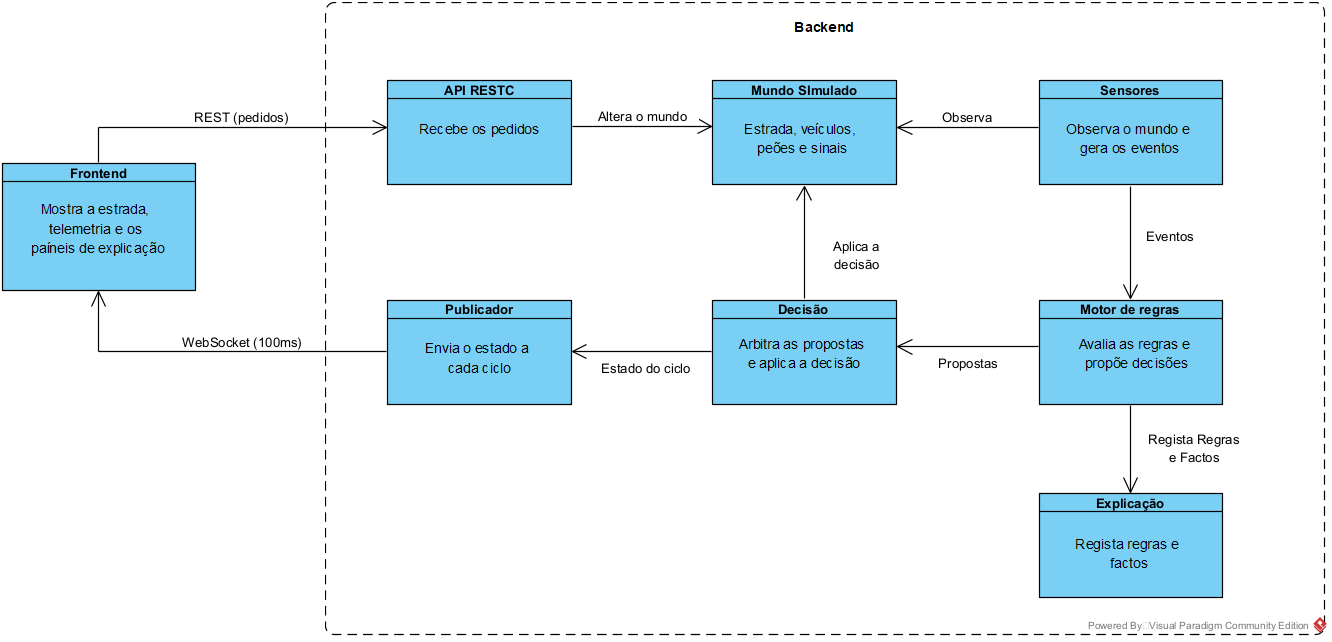
\includegraphics[width=\linewidth,height=0.80\textheight,keepaspectratio]{figuras/fig08_arquitetura_do_sistema_e_fluxo}
\caption{Arquitetura do sistema e fluxo de informação}\label{fig:8}
\end{figure}

\begin{tabela}{L{\dimexpr0.1797\linewidth-2\tabcolsep\relax}L{\dimexpr0.2994\linewidth-2\tabcolsep\relax}L{\dimexpr0.5189\linewidth-2\tabcolsep\relax}}
\caption{Tecnologias utilizadas}\label{tab:10}\\
\linhacab \cab{\textbf{Componente}} & \cab{\textbf{Tecnologia}} & \cab{\textbf{Utilização}} \\
\endfirsthead
\linhacab \cab{\textbf{Componente}} & \cab{\textbf{Tecnologia}} & \cab{\textbf{Utilização}} \\
\endhead
Backend & Java 17, Spring Boot 3.3.4 & Simulação, sensores, motor de inferência e API REST/WebSocket \\
\rowcolor{corFundo}Motor de regras & Drools / KIE 8.44 & Sessão com estado, regras DRL, CEP, encadeamento progressivo e consultas \\
Frontend & Angular 18, RxJS & Visualização da simulação e dos painéis do sistema pericial \\
\rowcolor{corFundo}Comunicação & WebSocket e REST & Estado em tempo real (WebSocket) e pedidos (REST) \\
Testes & JUnit 5, Jasmine/Karma, Playwright & Regras, arbitragem, ciclo de simulação, integração e testes de ponta a ponta \\
\end{tabela}

\section{O ciclo de simulação e organização do motor de inferência}\label{sec:6.2}

O ciclo de simulação tem por base intervalos de 100 ms, durante os quais são processadas as leituras dos sensores simulados, atualizada a informação disponível na memória de trabalho e avaliadas as regras aplicáveis. As decisões resultantes são utilizadas para atualizar o estado do veículo simulado, o que permite que as alterações do ambiente sejam consideradas nos ciclos seguintes, como representado na Figura~\ref{fig:9}, através da sequência das operações realizadas em cada ciclo.

\begin{figure}[H]
\centering
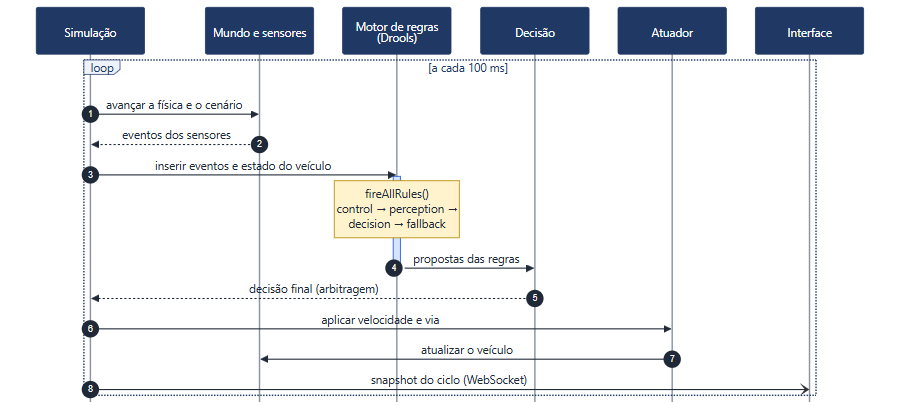
\includegraphics[width=0.94\linewidth,height=0.80\textheight,keepaspectratio]{figuras/fig09_sequencia_de_um_ciclo_de}
\caption{Sequência de um ciclo de simulação}\label{fig:9}
\end{figure}

Com o objetivo de organizar a informação recebida pelo motor de inferência \emph{Drools}, os eventos são encaminhados através de seis entry points, apresentados na Tabela~\ref{tab:11}. Esta organização permite separar os diferentes tipos de informação e identificar os fluxos relevantes para a avaliação das regras, incluindo aquelas que dependem de condições temporais.

\begin{tabela}{L{\dimexpr0.2852\linewidth-2\tabcolsep\relax}L{\dimexpr0.7128\linewidth-2\tabcolsep\relax}}
\caption{Entry points e eventos}\label{tab:11}\\
\linhacab \cab{\textbf{Entry point}} & \cab{\textbf{Eventos}} \\
\endfirsthead
\linhacab \cab{\textbf{Entry point}} & \cab{\textbf{Eventos}} \\
\endhead
VEHICLE\_STREAM & Velocidade do veículo \\
\rowcolor{corFundo}PERCEPTION\_STREAM & Distância, velocidade relativa e TTC; peões; ocupação das vias laterais; veículos nas vias vizinhas \\
ROAD\_STREAM & Sinais de limite de velocidade e de STOP, passadeiras, buracos, obstáculos, barreiras \\
\rowcolor{corFundo}TRAFFIC\_STREAM & Estado dos semáforos \\
ENVIRONMENT\_STREAM & Chuva, visibilidade e aderência \\
\rowcolor{corFundo}COMMAND\_STREAM & Pedidos de aceleração e de mudança de via \\
\end{tabela}

As regras são organizadas em quatro grupos, apresentados na Tabela~\ref{tab:12}. Esta divisão permite separar o processamento das perceções, a avaliação das condições de decisão e os comportamentos predefinidos quando nenhuma outra ação é proposta. A sequência de execução é coordenada por uma meta-regra de controlo, através da qual é estabelecida uma ordem entre as diferentes fases do processo de inferência.

\begin{tabela}{L{\dimexpr0.1496\linewidth-2\tabcolsep\relax}L{\dimexpr0.1398\linewidth-2\tabcolsep\relax}L{\dimexpr0.7086\linewidth-2\tabcolsep\relax}}
\caption{Grupos de agenda}\label{tab:12}\\
\linhacab \cab{\textbf{Grupo}} & \cab{\textbf{Nº de Regras}} & \cab{\textbf{Função}} \\
\endfirsthead
\linhacab \cab{\textbf{Grupo}} & \cab{\textbf{Nº de Regras}} & \cab{\textbf{Função}} \\
\endhead
control & 1 & Meta-regra responsável por coordenar a sequência de execução dos grupos de agenda \\
\rowcolor{corFundo}perception & 33 & Transformação de eventos em factos de estado, gestão da validade das perceções e avaliação da segurança das vias adjacentes \\
decision & 87 & Avaliação das condições e proposta de ações, assim como o tratamento das condições meteorológicas, o arranque e a ultrapassagem \\
\rowcolor{corFundo}fallback & 2 & Definição de comportamentos predefinidos quando não existem outras decisões aplicáveis \\
\end{tabela}

No que diz respeito ao tratamento das condições meteorológicas, é utilizada a lógica difusa para representar grandezas como a visibilidade e a aderência, na qual cada leitura pertence, com um grau entre 0 e 1, a vários conjuntos ao mesmo tempo, nomeadamente:

\begin{itemize}
  \item Conjuntos difusos: a visibilidade e a aderência partilham quatro conjuntos linguísticos, designados por fraca, reduzida, razoável e boa (Figura~\ref{fig:10}a). Os conjuntos sobrepõem-se e, em qualquer ponto, os graus de pertença somam 1, pelo que uma leitura pode ser, por exemplo, razoável com grau de 0,75 e reduzida com grau 0,25. A saída é a velocidade máxima recomendada, descrita por cinco conjuntos: muito lenta, lenta, moderada, prudente e ligeira (Figura~\ref{fig:10}b).
\end{itemize}

\begin{figure}[H]
\centering
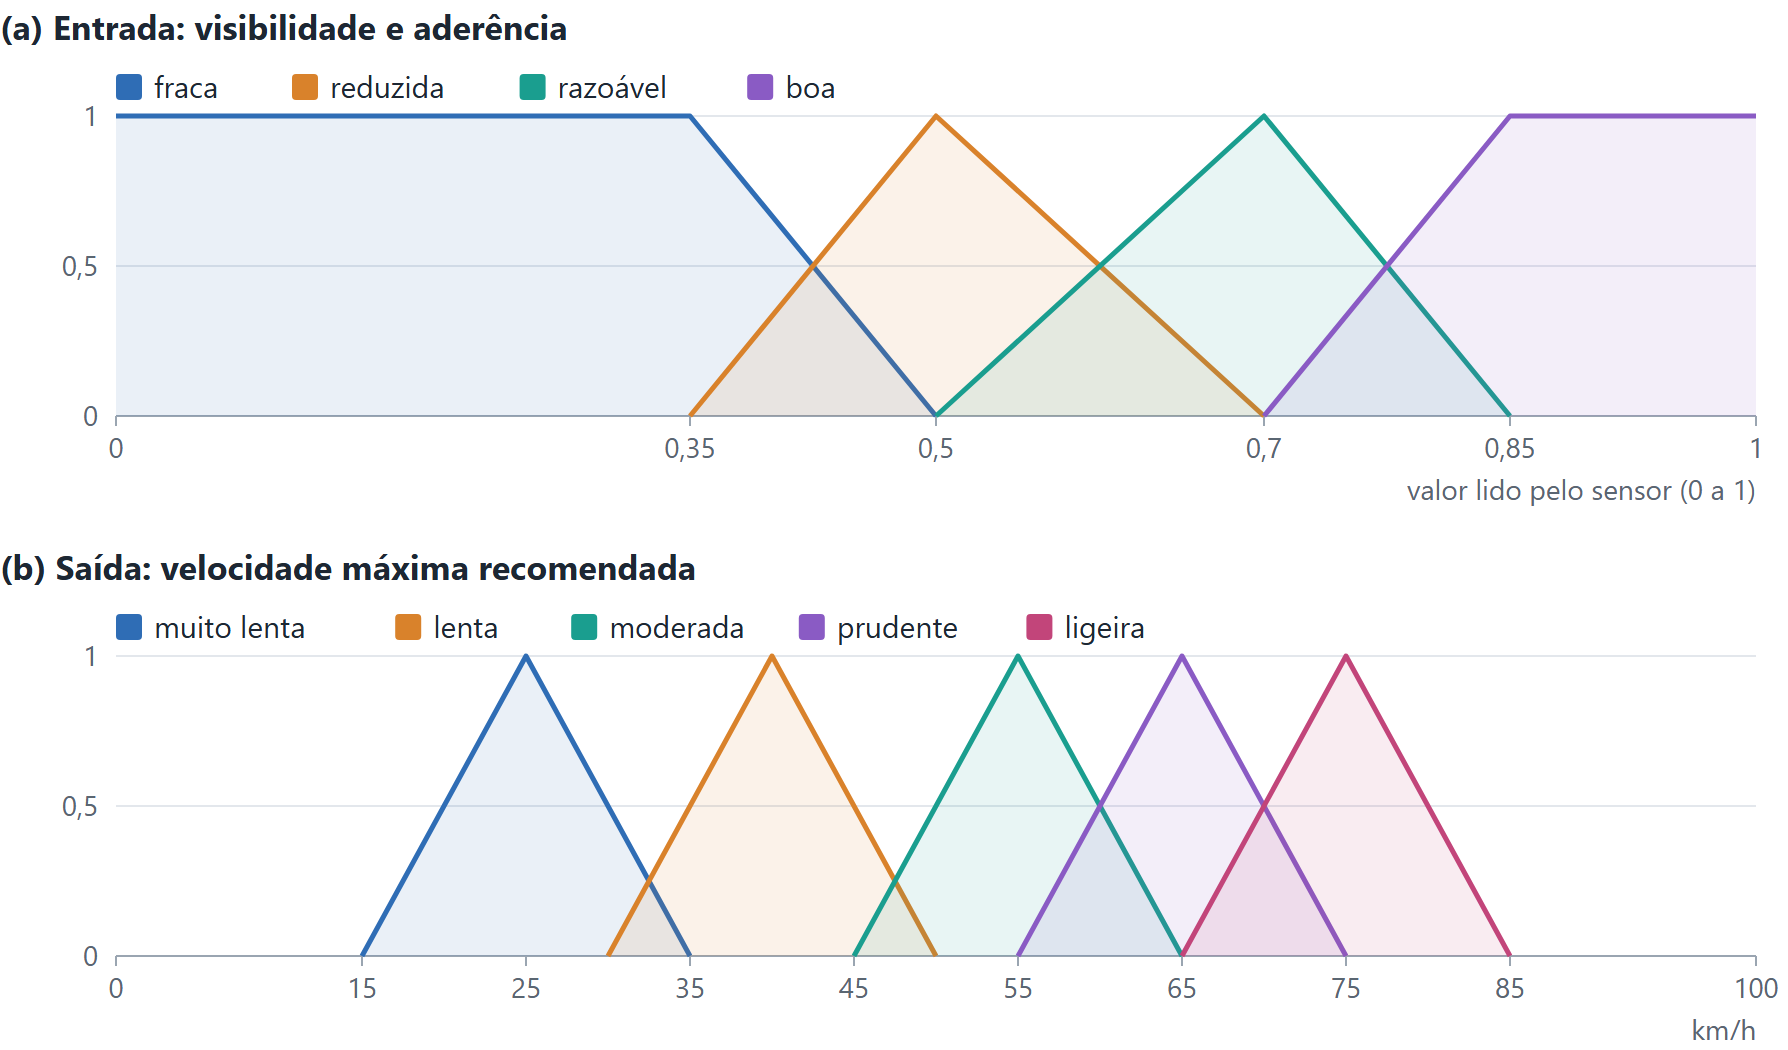
\includegraphics[width=0.89\linewidth,height=0.80\textheight,keepaspectratio]{figuras/fig10_conjuntos_difusos_a_visibilidade}
\caption{Conjuntos difusos: (a) visibilidade e aderência e (b) velocidade máxima recomendada}\label{fig:10}
\end{figure}

\begin{itemize}
  \item Regras difusas: As duas grandezas são combinadas, através de cinco regras (Tabela~\ref{tab:13}). As três primeiras utilizam a disjunção (OU), calculada pelo máximo, uma vez que basta uma das grandezas estar degradada para justificar a redução da velocidade. As duas últimas utilizam a conjunção (E), calculada pelo mínimo, e aplicam-se apenas quando ambas são boas, situação em que a chuva distingue uma velocidade prudente de uma velocidade ligeira.
\end{itemize}

\begin{tabela}{L{\dimexpr0.0924\linewidth-2\tabcolsep\relax}L{\dimexpr0.5482\linewidth-2\tabcolsep\relax}L{\dimexpr0.3574\linewidth-2\tabcolsep\relax}}
\caption{Regras difusas da meteorologia}\label{tab:13}\\
\linhacab \cab{\textbf{Regra}} & \cab{\textbf{SE}} & \cab{\textbf{ENTÃO velocidade}} \\
\endfirsthead
\linhacab \cab{\textbf{Regra}} & \cab{\textbf{SE}} & \cab{\textbf{ENTÃO velocidade}} \\
\endhead
1 & visibilidade fraca OU aderência fraca & muito lenta \\
\rowcolor{corFundo}2 & visibilidade reduzida OU aderência reduzida & lenta \\
3 & visibilidade razoável OU aderência razoável & moderada \\
\rowcolor{corFundo}4 & chuva E visibilidade boa E aderência boa & prudente \\
5 & sem chuva E visibilidade boa E aderência boa & ligeira \\
\end{tabela}

\begin{itemize}
  \item Aplicação no Drools: Uma vez que o Drools não tem suporte nativo para a lógica difusa, o controlador foi implementado através das regras do grupo \emph{decision}, com o apoio da classe \emph{FuzzySupport}. A fuzzificação converte as leituras em graus de pertença, que são, posteriormente, utilizados pelas regras para produzir as conclusões difusas. Tanto os graus de pertença como as conclusões são inseridos através do \emph{insertLogical}, o que permite ao \emph{Drools} removê-los automaticamente quando as leituras meteorológicas mudam. A título de exemplo, com chuva, visibilidade de 0,7 e aderência de 0,65, a visibilidade é razoável com grau 1 e a aderência é razoável com grau 0,75 e reduzida com grau 0,25. Assim, a regra 3 dispara com grau 1, conclui com velocidade moderada, e a regra 2 com grau 0,25, conclui com velocidade lenta. O centroide da área resultante é de 50,6 km/h, ou seja, aproximadamente 51 km/h, um valor próximo da velocidade moderada, mas reduzido pela contribuição da velocidade lenta (Figura~\ref{fig:11}).
\end{itemize}

\begin{figure}[H]
\centering
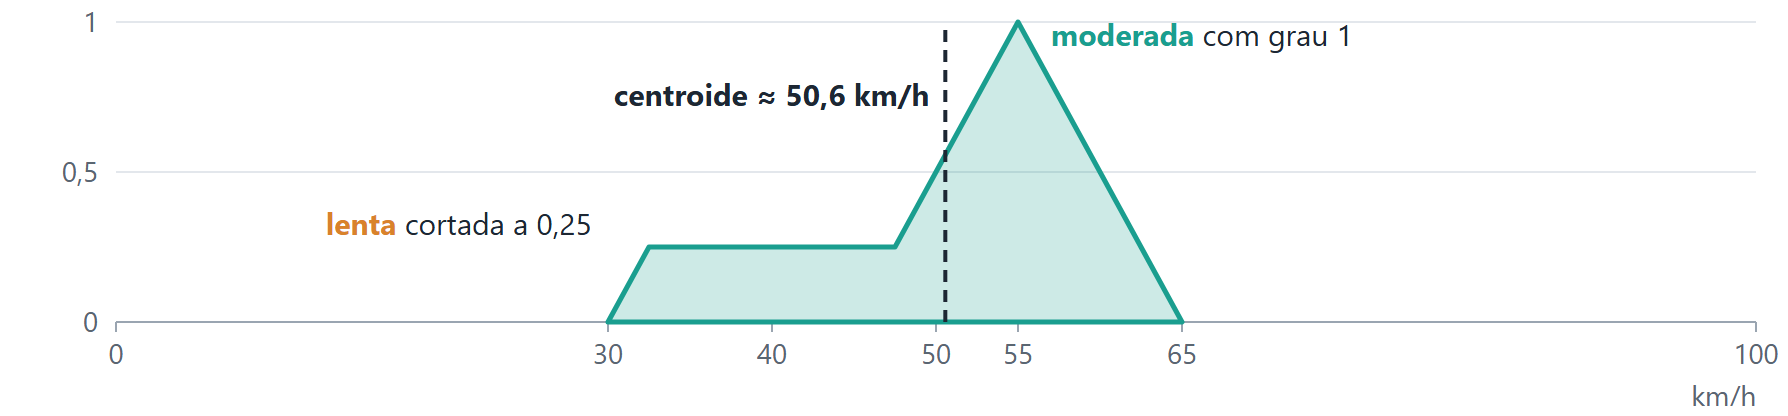
\includegraphics[width=0.89\linewidth,height=0.80\textheight,keepaspectratio]{figuras/fig11_exemplo_com_chuva_visibilidade_0}
\caption{Exemplo com chuva, visibilidade 0,7 e aderência 0,65}\label{fig:11}
\end{figure}

Desta forma, a organização dos fluxos e dos grupos permite estruturar o processo de inferência, enquanto a utilização das regras temporais e difusas possibilita considerar a evolução das condições observadas durante a simulação.

\section{Comunicação em tempo real: WebSocket}\label{sec:6.3}

A interface tem de mostrar, dez vezes por segundo, o veículo, as deteções, as decisões de velocidade e de via, a linha temporal e a memória de trabalho. Para isso, o backend mantém uma ligação WebSocket com o browser e envia, a cada ciclo, um snapshot JSON completo do sistema, num só sentido, do backend para o frontend. Como o snapshot inclui a decisão, as propostas, a evidência, a memória de trabalho e a linha temporal, a explicação de cada ciclo chega à interface sem cálculo adicional. Os comandos seguem por REST, porque cada um precisa da sua própria resposta e código de erro, e o backend envia um snapshot logo a seguir a cada comando, para que o efeito seja visível sem esperar pelo ciclo seguinte (Tabela~\ref{tab:14}). A ligação só é aceite a partir da origem da interface do projeto; as restantes são rejeitadas (403).

\begin{tabela}{L{\dimexpr0.5267\linewidth-2\tabcolsep\relax}L{\dimexpr0.4713\linewidth-2\tabcolsep\relax}}
\caption{Canais de comunicação}\label{tab:14}\\
\linhacab \cab{\textbf{Função}} & \cab{\textbf{Canal}} \\
\endfirsthead
\linhacab \cab{\textbf{Função}} & \cab{\textbf{Canal}} \\
\endhead
Ciclo de vida (iniciar, pausar, parar, reiniciar) & REST \\
\rowcolor{corFundo}Carregar cenários & REST \\
Alterar o mundo (elementos, meteorologia) & REST \\
\rowcolor{corFundo}Consultar viagens e perguntas Why / Why Not / How & REST \\
Estado em tempo real & WebSocket \\
\end{tabela}

A publicação do estado não pode atrasar a inferência. Por isso, cada cliente tem um emissor próprio e uma única posição de espera, que guarda apenas o snapshot mais recente: um browser lento salta estados intermédios, mas como cada snapshot é completo nunca fica com informação errada, e o ciclo de 100 ms mantém-se inalterado. Se a ligação falhar, o frontend deteta a falha e restabelece-a automaticamente.

\section{Cenários}\label{sec:6.4}

Foram definidos cenários pré-construídos que abrangessem um pouco de todo o sistema. Neste sentido, a título de exemplo, apresenta-se a traçagem do cenário de TTC crítico com chuva, na Tabela~\ref{tab:15}. Para este cenário considera-se que o veículo segue a 95 km/h na via do meio, com outro a 30 km/h 40 m à frente (TTC ≈ 2,2 s).

\begin{tabela}{L{\dimexpr0.0741\linewidth-2\tabcolsep\relax}L{\dimexpr0.3513\linewidth-2\tabcolsep\relax}L{\dimexpr0.1671\linewidth-2\tabcolsep\relax}L{\dimexpr0.2078\linewidth-2\tabcolsep\relax}L{\dimexpr0.1977\linewidth-2\tabcolsep\relax}}
\caption{Traçagem do cenário TTC crítico com chuva}\label{tab:15}\\
\linhacab \cab{t} & \cab{Perceção e estado} & \multicolumn{2}{L{\dimexpr0.3749\linewidth-2\tabcolsep\relax}}{\cab{Propostas de decisão}} & \cab{Decisão aplicada} \\
\endfirsthead
\linhacab \cab{t} & \cab{Perceção e estado} & \multicolumn{2}{L{\dimexpr0.3749\linewidth-2\tabcolsep\relax}}{\cab{Propostas de decisão}} & \cab{Decisão aplicada} \\
\endhead
0,1 s & 1.ª leitura de TTC: ainda não há janela; lógica difusa (Mamdani) com insertLogical dá ≈ 51 km/h & \textbf{WON} & Keep safe following distance...: 48 km/h · p50. & Vence o teto mais baixo;\par a ultrapassagem inicia-se \\*
 &  & \textbf{LOST\_TO} & Defuzzify weather speed ceiling: 51 km/h · p40. &  \\*
 &  & \textbf{WON} & Overtake slow front vehicle via left lane · p30 &  \\
\rowcolor{corFundo}0,2 s & 2 leituras de TTC < 3 s em 2 s, cada uma coincide[400ms] com uma leitura de chuva & \textbf{WON} & Persistent low TTC in rain increases conservatism: BRAKE 15 km/h · p50 & \textbf{Trava; }\par \textbf{manobra em curso} \\
0,3 s & accumulate ... over window.time(2s): 3 leituras de TTC < 2,5 s (mínimo 1,94 s) & \textbf{WON} & Emergency brake when persistent TTC is critical · p70. & \textbf{−8,5 m/s² e luzes de emergência; }\par \textbf{a manobra já iniciada não é abortada} \\*
 &  & \textbf{LOST\_TO} & chuva, seguimento, aproximação, difusa, cruzeiro &  \\*
 &  & \textbf{VETOED\_BY} & Maintain ongoing lane change left (anulada) &  \\
\rowcolor{corFundo}3,1 s & Manobra concluída: via da esquerda, sem veículo à frente & \textbf{WON} & Defuzzify weather speed ceiling: 51 km/h · p40 & Acelera de 10 até ≈ 51 km/h \\
\end{tabela}
